\chapter{ZI-Round extensions} \label{ch:ziroundextensions}
In this thesis the implementation of ZI-Round that takes the singletons into account and employs the extension of improving the objective value by shifting non-fractional integer variables while rounding the fractional ones is referred to as the default version, i.e. the one described in Chapter~\ref{ch:ziround}. \par
In this chapter, some variations and extensions of the ZI-Round heuristic are presented, together with some example charts showing the behavior of the solution cost and fractionality as the inner loop iterations of ZI-Round progress. Note that only one feature at a time is changed from the default ZI-Round implementation: all the features of default ZI-Round are kept, except for the one changed by each extension.
Eventually, a new default version of ZI-Round is proposed. \par 
The charts presented are made by the author of this thesis using the Gnuplot graphing utility \cite{gnuplot}, called directly from the main program through a pipe. The data portrayed by the charts is obtained from the experiments conducted, which are described in detail in Chapter~\ref{ch:compresults}.

\section{Default ZI-Round} \label{sec:default}
The default version of ZI-Round shifts both fractional and non-fractional integer variables, the latter to improve the objective value.
The two phases of rounding and objective improvement are overlapped, causing the solution cost to vary unsteadily until all the fractional integer variables have been rounded. The rounding phase terminates when the solution fractionality reaches zero and from that point on the objective improvement phase continues until no more improvements are possible.
A visual example of such behavior is shown in Figure~\ref{fig:exzi-default} for the instance \texttt{fast0507}: the two phases coexist until the solution fractionality reaches zero, at which point only the objective value improvement occurs.
\begin{figure}[ht]
	\centering
	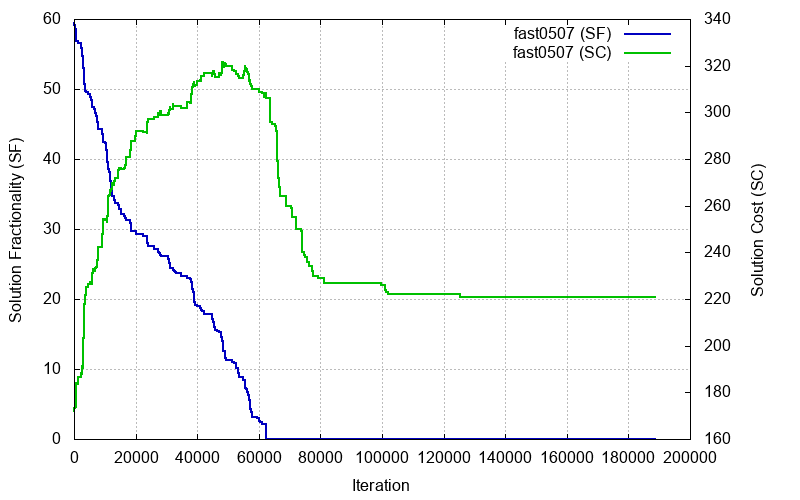
\includegraphics[width=\textwidth]{fast0507-default.png}
	\caption{ZI-Round execution for the instance \texttt{fast0507}: default.}
	\label{fig:exzi-default}
\end{figure}

\section{Sorted singletons}
A first simple extension follows from a possible improvement on the order in which the singletons of a given constraint are considered when distributing the singletons slack on them, with the aim of worsening the objective value as little as possible. \par 

In the default implementation of ZI-Round the singletons are considered in their natural order. The proposed improvement consists in sorting the singletons of each constraint in ascending order of their objective function coefficients, so that the first singleton variables to be updated are the ones that affect the objective value the least. \par

We recognize that this greedy approach does not ensure to always affect the objective value in a positive way, since the current possible singleton variations would need to be taken into account at each iteration, and those variations depend on the bounds of the singleton and its coefficient in the constraint. However, this simple extension is tested with the aim of showing whether and in what amount the order in which the singletons are considered influences the end results. The chosen reference instance does not have any singletons in its constraints, hence no example chart is available for this extension.

\section{No objective improvement}
Another extension of ZI-Round worth analyzing is the shift of non-fractional integer variables to improve the objective value as much as possible. Since this extension is part of the default version of ZI-Round, its complementary counterpart is considered, i.e. the absence of it. \par

The rationale behind this non-extension is the following. First, observe that the overall slack of a constraint can be viewed as its capacity to cover the possible shift of one of its variables, and a variable shift can either increase or decrease that capacity. Also, in a way, the constraints of a MIP should generally go against the objective function, otherwise the problem would be unbounded. It follows that shifting non-fractional integer variables to improve the objective value should contribute to the saturation of the shift coverage capacity of the constraints, which could not be able to allow all the fractional integer variables to be rounded. \par

This non-extension that avoids shifting non-fractional integer variables is tested with the aim of showing whether and in what amount the attempt to improve the objective value while rounding all the integer variables influences the end results, especially in terms of quality of the solutions found. \par

Without objective improvement, the rounding phase is free to operate and terminates as soon as the solution fractionality reaches zero, marking the end of the heuristic. A visual example of such behavior is shown in Figure~\ref{fig:exzi-noobjimprove} for the instance \texttt{fast0507}. Note that all the fractional integer variables are rounded after way less iterations with respect to the default version, which shows how the objective improvement phase interferes with the rounding phase, making the rounding process longer.
\begin{figure}[ht]
	\centering
	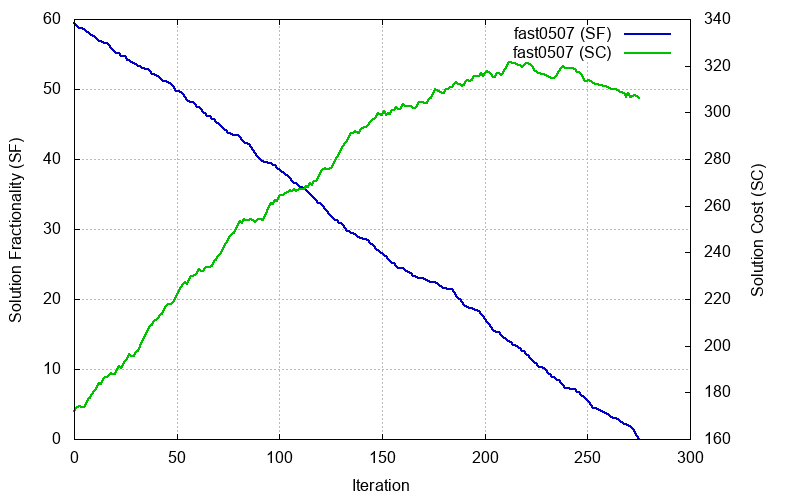
\includegraphics[width=\textwidth]{fast0507-noshiftnonfrac.png}
	\caption{ZI-Round execution for the instance \texttt{fast0507}: no objective improvement.}
	\label{fig:exzi-noobjimprove}
\end{figure}

\section{Objective improvement after zero fractionality}
The previous non-extension is a rather conservative approach that avoids any objective value improvement from start to finish. \par 

A very reasonable extension that allows the fractional integer variables to fully rely on the slacks in order to be rounded and the objective value to be improved consists in starting to shift the non-fractional integer variables only after all the fractional ones have been rounded. In other words, this extension would follow the previous one until the fractionality of the solution reaches zero or no more fractional variables can be rounded, and then start improving the objective value by shifting all the integer variables, which would all be non-fractional at that point. \par

This two-phased extension that first concentrates on rounding all the fractional integer variables and only after no more fractional variables can be rounded proceeds to improve the objective value is tested with the aim of showing whether and in what amount separating the rounding phase and the objective improvement phase affects the end results. \par 

Since the two phases are separated, at first all the slacks are exclusively at the disposal of the rounding phase, which is prioritized. This separation is reflected in the behavior of the solution cost, which tends to increase while the fractionality approaches zero, at which point the objective improvement phase starts shifting the non-fractional integer variables, causing the objective value to decrease until no more improvements are possible. A visual example of such behavior is shown in Figure~\ref{fig:exzi-objimproveafter0frac} for the instance \texttt{fast0507}. The rounding phase is the same as in Figure~\ref{fig:exzi-noobjimprove}, with the solution fractionality of the instance reaching zero at iteration $275$, at which point the objective improvement phase starts operating until the end of the heuristic.
\begin{figure}[ht]
	\centering
	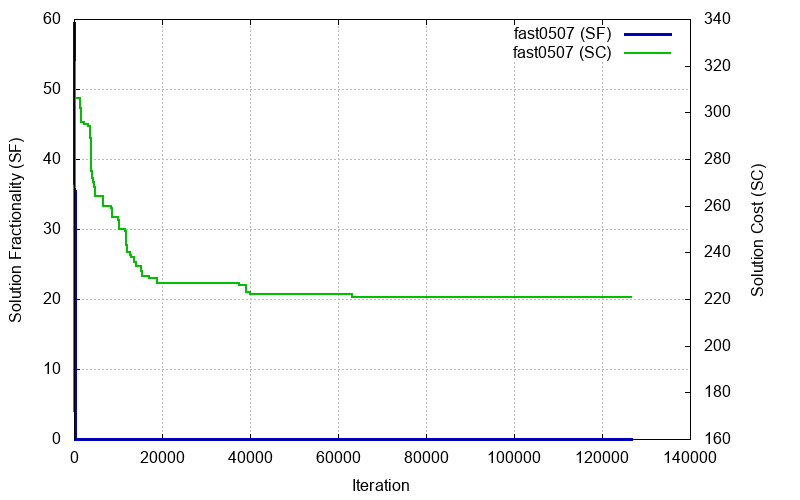
\includegraphics[width=\textwidth]{fast0507-shiftnfafter0frac.png}
	\caption{ZI-Round execution for the instance \texttt{fast0507}: objective improvement after zero fractionality.}
	\label{fig:exzi-objimproveafter0frac}
\end{figure}

\section{Worst-objective fractionality tie-breaks}
The final extension proposed follows from the observation that any attempt at improving the objective value generally goes against the capacity of the constraints to compensate for the shifts of the variables they contain. \par 

As reported in Algorithm~\ref{alg:ziround}, the default behavior of ZI-Round when fractionality tie-breaks occur during the rounding process of a fractional integer variable is to prefer the rounding direction that improves the objective value the most, or worsens it the least. This proposed extension, instead, in such cases would choose to round the variable in the direction that worsens the objective value the most, or improves it the least. This behavior would in fact favor the constraints, thus the possibility of rounding more fractional integer variables. \par

Note that the shifting of non-fractional integer variables of the default ZI-Round implementation is maintained. This mixed extension that favors both the objective function and the constraints is tested with the aim of showing whether and in what amount favoring the constraints when either direction can be chosen while rounding a fractional integer variable affects the end results. \par 

Since the direction that worsens the objective value is chosen whenever a tie on the fractionality improvement given by a possible shift occurs, in such cases more power is given to the rounding phase. On the other hand, the objective improvement phase still operates concurrently throughout the execution of the heuristic. A visual example of such behavior is shown in Figure~\ref{fig:exzi-fractieworstobj} for the instance \texttt{fast0507}: as expected, it is similar to the one obtained by the default version of ZI-Round, since the two phases still interfere with one another from the start.
\begin{figure}[ht]
	\centering
	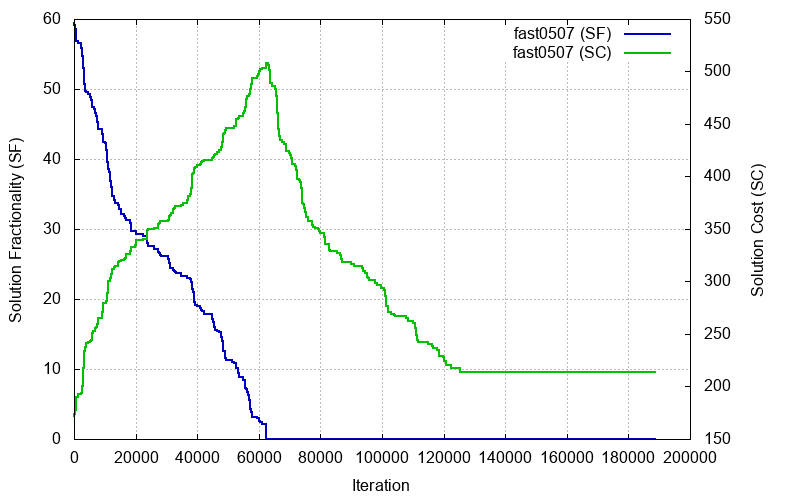
\includegraphics[width=\textwidth]{fast0507-fractieworstobj.png}
	\caption{ZI-Round execution for the instance \texttt{fast0507}: worst-objective fractionality tie-breaks.}
	\label{fig:exzi-fractieworstobj}
\end{figure}

\section{Proposed ZI-Round} \label{sec:proposed}
From the behaviors of the extensions observed and the experiments conducted, the following version of ZI-Round is proposed as the new default. The proposed ZI-Round heuristic employs the sorting of the singletons of each constraint, the worst-objective fractionality tie-breaks and the objective improvement after the fractionality reaches zero. The experimental results that support this choice are presented in Chapter~\ref{ch:compresults}. \par
The behavior of the solution cost and fractionality for the instance \texttt{fast0507} under the proposed version of ZI-Round is shown in Figure~\ref{fig:exzi-proposed}. Unlike in Figure~\ref{fig:exzi-objimproveafter0frac}, where the final objective value is $221$, in this case a solution with an objective value of $214$ is found.
\begin{figure}[ht]
	\centering
	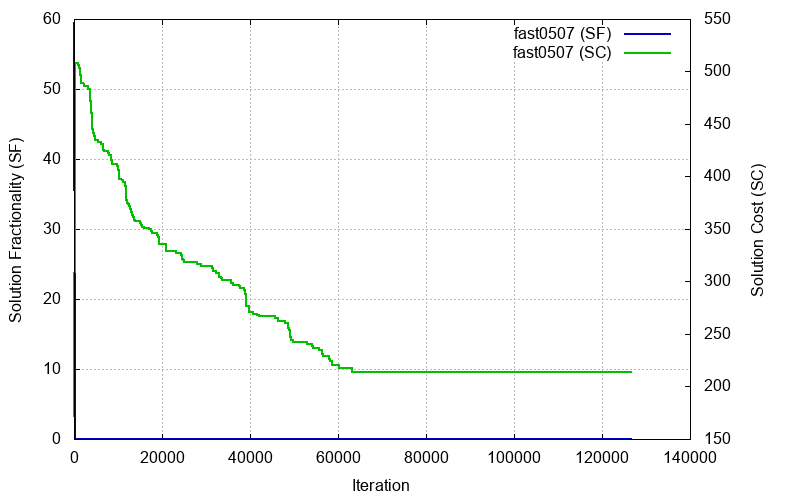
\includegraphics[width=\textwidth]{fast0507-proposed.png}
	\caption{ZI-Round execution for the instance \texttt{fast0507}: proposed.}
	\label{fig:exzi-proposed}
\end{figure}